\documentclass[]{article}

\usepackage[polish]{babel}
\usepackage{amsmath}
\usepackage{amsfonts}
\usepackage{amssymb}
\usepackage[T1]{fontenc}
\usepackage[toc]{glossaries}
\usepackage{graphicx}
\usepackage{float}


%opening
\title{{\normalsize Sprawozdanie IV} \\
		{\Huge Algorytmy z powracaniem}}
\author{Piotr Tylczyński}
\date{31 maja 2019}

\makeglossaries
\newglossaryentry{m}
{
	name={m},
	description={ilość krawędzi w grafie}
}

\newglossaryentry{G}
{
	name={G},
	description={Spójny, nieskierowany graf}
}

\newglossaryentry{n}
{
	name={n},description={ilość krawedzi}
}

\begin{document}

\maketitle
\clearpage

\tableofcontents
\clearpage

\section{Nieskierowany cykl Eulera}
	\subsection{Opis}
		Jest to taki cykl w grafie nieskierowanym, w którym da się przejść przez wszystkie krawędzie tego grafu, tak aby przez każdą krawędź przejść dokładnie raz. \\
		Cykl taki będzie istniał o ile każdy wierzchołek będzie miał parzysty stopień.
	
	\subsection{Złożoność algorytmu}
		\begin{figure}[H]
			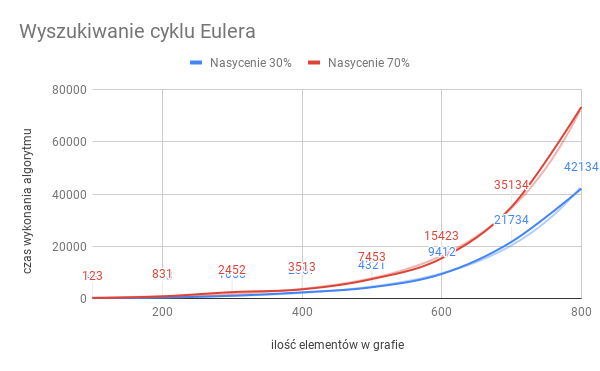
\includegraphics[scale=0.6]{euler.png}
		\end{figure}
		\paragraph{Wybór reprezentacji}
		Do zaimplementowania grafu została użyta tablica krawędzi. Taka reprezentacja gwarantuje stałą złożonośc czasową operacji stwierdzenia istnienia krawędzi, oraz liniową złożoność operacji wyszukiwania następników danegow wierzchołka.
		
		\paragraph{Opis działania algorytmu} Pierwszym krowkiem wykonania algorytmu jest wskazanie wierzchołka początkowego, wybór ten nie ma wpływu na powodzenie, lub nie wykonania algorytmu. Następnie algorytm korzystając z metody przeszukiwania grafu wszerz przechodzi przez wszystkie krawędzie, jednocześnie usuwając te, przez które przeszedł, oraz zapisując je do struktury wynikowej.
		
		\paragraph{Złożoność czasowa}
		Na złożoność czasową algorytmu mają wpływ
		\begin{itemize}
			\item ilość krawędzi
			\item złożoność czasowa wyszukiwania następników
		\end{itemize}
		Złożonośc czasowa to:
		\begin{equation}
			O(mn)
		\end{equation}
		Wynika ona z:
		\begin{gather}
			\text{ilość operacji} = \text{czas szukania wszytskich następników} * \text{ilość wierzchołków} \\
			\text{ilość operacji} = n * n
		\end{gather}
		
\clearpage
\section{Nieskierowany cykl Hamiltona}
	\subsection{Opis}
		Jest to atki cykl w grafie nieskierowany, który pozwala przejśc przez wszystkie wierzchołki grafu dokładnie raz. \\
		Niestety w przeciwieństwie do nieskierowanego grafu Eulera, nie znaleźono jeszcze prostej metody na określenie istnienia nieskierowanego cyklu Hamiltona.
		
	\subsection{Złożonośc algorytmu}
		\begin{figure}[H]
			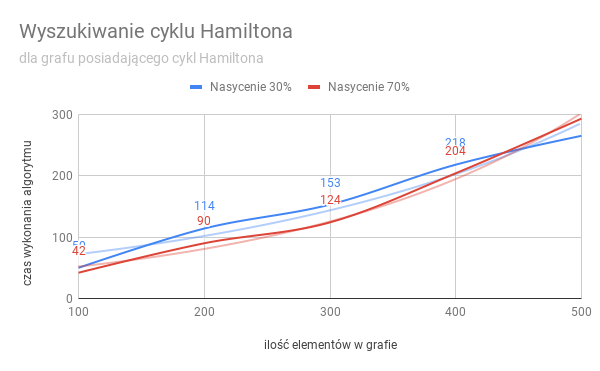
\includegraphics[scale=0.6]{hamilton.png}
			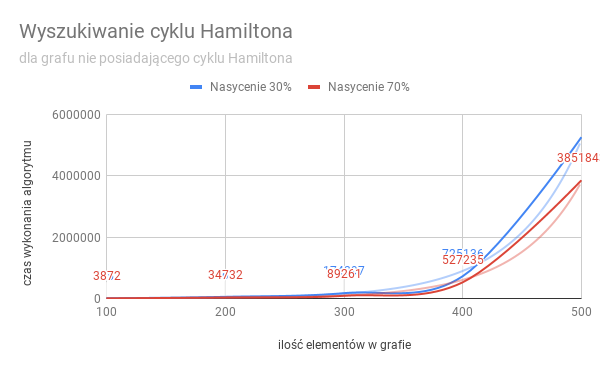
\includegraphics[scale=0.6]{hamiltonwo.png}
		\end{figure}
		\paragraph{Wybór reprezentacji}
		Do zaimplementowania grafu została użyta tablica krawędzi. Taka reprezentacja gwarantuje stałą złożonośc czasową operacji stwierdzenia istnienia krawędzi, oraz liniową złożoność operacji wyszukiwania następników danegow wierzchołka.
		
		\paragraph{Opis działania algorytmu}
		Pierwszym krokiem jest wskazania wierzchołka, od którego algorytm zacznie swoje wykonanie. Tak samo jak w poprzednim przypadku wybór wierzchołka nie ma wpływu na powodzenie lub nie wykonania algorytmu. Następnie algorytm odwiedza wszystkie wierchołki incydentne z wierchołkiem, w którym się znajduje, jednocześnie oznaczając wierchołki, które przebył jako odwiedzone. W momencie, w który wszystkie wierzchołki zostały odwiedzone zostaje sprawdzone czy ostatni wierzchołek, w który znajdował się algorytm jest połączony z wierzchołkiem, z którego algorytm rozpoczynał swoje działanie, jeśli tak jest ścieżka jaką przebył algorytm jest poszukiwanym cyklem Hamiltona. W przeciwnym wypadku należy cofnąć algorytm do momentu w którym istnieje możliwość wyboru innego wtedy jeszcze nieodwiedzonego wirchołka i wykonanie algorytmu od tego momentu jeszcze raz.
		
		\paragraph{Złożonośc czasowa}
		W najlepszym przypadku, czyli  w momencie, w którym graf będzie skaład się tylko i wyłącznie z krawędzi tworzących cykl to złożoność czasowa będzie wynosić:
			\begin{equation}
				O(n)
			\end{equation}
		Jednak w najgorszym przypadku, czyli gdy graf będzie pełny, złożność może wzrosnąć do:
			\begin{equation}
				O(n!)
			\end{equation}
		Wynika to z potrzby sprawdzenia wszytkich możliwych ułożeń $n$ wierzchołków, co w przypadku grafu pełnego może wymagać parmutacji bez powtórzeń $n$ elementów.
			

\clearpage
\glsaddall
\printglossaries

\end{document}
